\documentclass[10pt,twocolumn]{article}

\usepackage[utf8]{inputenc}
\usepackage[T1]{fontenc}
\usepackage{lmodern}
\usepackage{microtype}
\usepackage[margin=0.75in,columnsep=0.25in]{geometry}
\usepackage{amsmath,amssymb}
\usepackage{booktabs}
\usepackage{multirow}
\usepackage{array}
\usepackage{graphicx}
\usepackage[table]{xcolor}
\usepackage{tikz}
\usetikzlibrary{arrows.meta,positioning}
\usepackage[numbers,sort&compress]{natbib}
\usepackage{caption}
\captionsetup{font=small,labelfont=bf,skip=4pt}
\usepackage{enumitem}
\setlist{nosep,leftmargin=*}
\usepackage[colorlinks=true,linkcolor=blue!50!black,citecolor=blue!50!black,urlcolor=blue!50!black]{hyperref}
\usepackage[capitalise,noabbrev]{cleveref}

\setlength{\textfloatsep}{10pt plus 2pt minus 2pt}
\setlength{\intextsep}{8pt plus 2pt minus 2pt}
\renewcommand{\topfraction}{0.9}
\renewcommand{\textfraction}{0.1}
\renewcommand{\floatpagefraction}{0.8}

\newcommand{\topk}{top-$k$}
\newcommand{\best}[1]{\cellcolor{blue!8}#1}
\newcommand{\up}{$\uparrow$}
\newcommand{\down}{$\downarrow$}
\newcommand{\ci}[2]{{\scriptsize[#1--#2]}}

\title{Detecting Weight Tampering in Verifiable LLM Inference:\\Per-Layer Activation Profiles and the Attention-Kernel Loophole}
\author{
  Vignesh Kanike\\
  Indian Institute of Technology Delhi\\
  \texttt{ms1240669@iitd.ac.in}
}
\date{}

\begin{document}
\maketitle

\begin{abstract}
Clients of inference providers usually cannot tell whether the open-weight model they paid for was run, or a cheaper quantised or fine-tuned copy.
TOPLOC (Ong et al., ICML 2025) lets a provider commit to the largest entries of the last hidden state, which a validator checks with one prefill, using thresholds loose enough to absorb honest numerical noise.
On Qwen2.5-1.5B-Instruct we find that this tolerance is the weak point: serving the reference model with eager attention changes the last layer more than 8-bit or 4-bit quantisation, so thresholds that accept it flag no quantised sequence and 55--60\% of fine-tuned ones.
Kernel noise and weight changes differ across depth, and a linear classifier on TOPLOC's statistics at all 28 layers attributes four known modifications with 99.3\% balanced accuracy (99.0\% from decode-time activations), against 78.0\% from the last layer alone.
We then test it as an integrity check against three kinds of provider.
It is not one in general: 8-bit quantisation left out of training is accepted on every test prompt, and a provider that serves quantised weights with eager attention is accepted on 92\% (8-bit) and 68\% (4-bit) of prompts at a 1\% false-rejection target.
With the kernel enforced to SDPA, no tampered model served on it was accepted: not the four known modifications at batch 1 or 4, six unseen partial or combined modifications, or a detector-guided choice of layers to quantise (0 of 50 per case).
On a second model, SmolLM2-1.7B, eager noise is small, the last layer alone suffices, and the loophole does not appear.
A per-layer TOPLOC commitment costs 57.8\,kB per 256 tokens.
Neither check binds the served text to the weights that generated it, so the results bound what activation checks can establish rather than provide an integrity guarantee.
\end{abstract}

%=====================================================================
\section{Introduction}
\label{sec:intro}

Open-weight language models are now served by many third parties: commercial APIs, decentralised compute networks and peer-to-peer inference markets.
A client names a model and pays per token, but it sees only text.
A provider that quantises the model or swaps in a fine-tuned copy saves memory or compute, and the text still reads well.
Gao et al.~\cite{gao2025model} tested 31 commercial endpoints for four Llama models and found 11 serving a different output distribution from the published weights.

TOPLOC~\cite{ong2025toploc} offers a cheap check.
Every 32 tokens the provider commits to the 128 largest entries of the last hidden state, and a validator recomputes them in a single prefill.
Because bf16 arithmetic differs slightly between GPUs and kernels, the validator accepts small exponent and mantissa disagreements and flags a sequence only above fixed thresholds.
That tolerance is where the difficulty lies.
A verifier has to accept every authorised execution, including honest providers on different kernels, and reject every unauthorised one.
If honest variation and weight tampering produce disagreements of the same size, no threshold does both.

We find exactly this overlap on Qwen2.5-1.5B-Instruct.
Serving the reference model with eager attention, a kernel TOPLOC did not evaluate, changes the last layer about six times as much as a batch-size change and more than 8-bit or 4-bit quantisation.
With thresholds calibrated to accept eager traffic, the check flags no quantised sequence and 55--60\% of fine-tuned ones.

\begin{figure*}[!t]
\centering
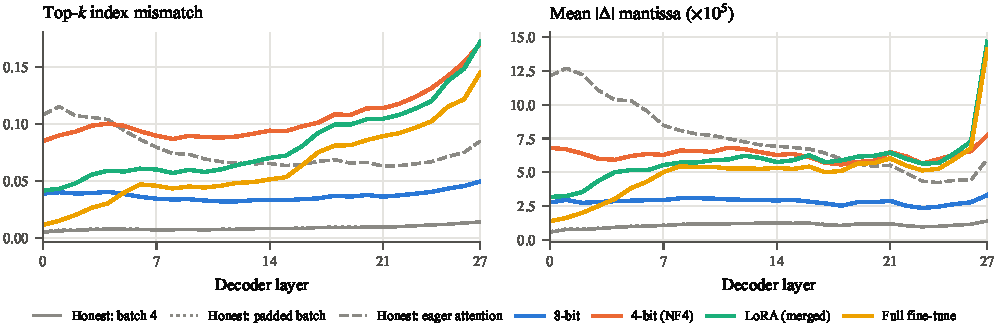
\includegraphics[width=\linewidth]{figures/profiles.pdf}
\caption{Kernel noise and weight changes peak at different depths. Mean \topk{} disagreement with the reference model at each decoder layer (Qwen2.5-1.5B-Instruct, 200 prompts). Grey lines are honest serving configurations; coloured lines are tampered weights. At layer 27, eager-attention noise sits among the quantised models; in the early layers it stands apart.}
\label{fig:profiles}
\end{figure*}

The two sources do differ in where they appear (\cref{fig:profiles}).
Eager-attention noise is largest in the first layers and fades with depth, quantisation shifts every layer by about the same amount, and fine-tuning grows toward the output.
We compute TOPLOC's statistics at all 28 layers and train a linear classifier on the resulting profile.
On the four modifications we trained on, it identifies the modification with 99.3\% balanced accuracy while accepting both kernels.

That number answers a narrower question than integrity verification, and most of this paper is about the gap.
We evaluate the profile against three kinds of provider (\cref{sec:threat}): one that tampers without regard to the detector, one that also chooses its kernel and batch size, and one that uses the detector's own score to choose what to quantise.
We also test modifications the classifier never saw, report false acceptance and false rejection rates at a fixed operating point with intervals, and separate what our implementation checks from what a deployed protocol would still have to guarantee.

Our findings, each tested in \cref{sec:results}:
\begin{itemize}
  \item With thresholds calibrated on mixed honest kernels, TOPLOC's last-layer check misses 8-bit and 4-bit quantisation and about half of light fine-tuning in our setup (\cref{sec:res-baseline}).
  \item The per-layer profile identifies four \emph{known} modifications with 99.3\% balanced accuracy, 99.0\% from decode-time activations, and most of its signal lies in the early and middle layers (\cref{sec:res-profile,sec:res-ablation,sec:res-decode}).
  \item It does not establish integrity against unknown modifications: 8-bit quantisation left out of training is accepted as clean on every test prompt (\cref{sec:res-open}).
  \item A provider that serves quantised weights with eager attention passes as honest on most prompts, even when the verifier uses a detector specific to the declared kernel. With the kernel enforced, no tested attack was accepted (\cref{sec:res-attack}).
  \item Six modifications never seen in training, including LoRA with 4-bit weights and partial quantisation, and a detector-guided choice of layers to quantise were all rejected with the kernel enforced; on SmolLM2-1.7B the kernel loophole does not appear and the last layer alone suffices, so both the problem and the benefit are model-dependent (\cref{sec:res-open,sec:res-aware,sec:res-smol}).
  \item A real per-layer TOPLOC commitment costs 57.8\,kB per 256 tokens and 0.5\,s of CPU time per sequence, and at batch 32 4-bit decoding reaches 96\% of bf16 throughput with less memory (\cref{sec:res-cost}).
\end{itemize}
Code and result files are at \url{https://github.com/bruce249/proof-of-weights}.

%=====================================================================
\section{Background and related work}
\label{sec:related}

\paragraph{TOPLOC.}
TOPLOC~\cite{ong2025toploc} records the last hidden state at one position per 32 decode steps, keeps its $k{=}128$ largest-magnitude entries, and encodes them in a polynomial commitment of a few hundred bytes.
The validator prefills the prompt and the claimed output with the committed weights, counts exponent mismatches between corresponding values, and takes the mean and median mantissa difference.
A sequence fails if the largest value of any statistic across its checkpoints exceeds a threshold; the published thresholds are $T_{\exp}{=}38$, $T_{\text{mean}}{=}10$ and $T_{\text{median}}{=}8$.
Its robustness tests covered A100 and RTX 4090 GPUs, Flash Attention 2, SDPA and FlexAttention, and tensor parallelism on Llama-3.1-8B and larger models, with no false positives~\cite[\S5.6, Table~2]{ong2025toploc}.
It did not test quantisation, notes that small fine-tuning updates are harder to detect~\cite[\S6.5]{ong2025toploc}, and cannot detect speculative decoding~\cite[\S6.2]{ong2025toploc}.

\paragraph{Statistical detection versus proof.}
Zero-knowledge proofs of inference such as zkLLM~\cite{sun2024zkllm} establish that a specific computation was performed, at minutes per query for a 13B model; SafetyNets~\cite{ghodsi2017safetynets} uses interactive proofs for smaller networks.
Trusted execution~\cite{tramer2019slalom,cai2025auditing} instead relies on the hardware vendor.
TOPLOC and the method in this paper are statistical tests: they bound how far observed activations may deviate from a recomputation, and their guarantees are only as strong as the separation between honest and dishonest deviations, which is what we measure.

\paragraph{Detecting substitution.}
Model equality testing~\cite{gao2025model} compares output text with a two-sample test; Cai et al.~\cite{cai2025auditing} show such tests need many queries and that log-probability tests are confused by nondeterministic inference.
SVIP~\cite{sun2025svip} trains a proxy task on returned hidden states to detect substitution with a smaller model.
These methods target swaps between different models, whereas we study quantisation and fine-tuning of the same model.

\paragraph{Nondeterminism and enforcement.}
Inference is not bitwise reproducible across batch sizes, padding and kernels~\cite{he2025nondeterminism}, so every activation check needs some tolerance.
Optimistic protocols such as Truebit~\cite{teutsch2019truebit} and opML~\cite{conway2024opml} accept results by default and settle disputes on challenge; TOPLOC has no stake or penalty.

%=====================================================================
\section{Threat model and problem}
\label{sec:threat}

\paragraph{Assets and parties.}
The asset is the client's assurance that a response was produced by the committed weights $\theta$, a model repository at a pinned revision.
A \emph{provider} stakes tokens, serves requests and posts a commitment for each response.
A \emph{validator} samples commitments, recomputes activations with $\theta$, and resolves challenges.
We trust the validator to run $\theta$ and to report its verdict honestly.
The contract enforces the stake, the bond and the dispute window; it does not check the verdict.

\paragraph{Authorised variation.}
An honest provider runs $\theta$ but may use a different attention kernel, batch size or padding from the validator.
In our experiments the authorised set is SDPA at batch 1 (the validator's own setting), eager attention at batch 1, SDPA at batch 4, and SDPA at batch 4 with extra padding.

\paragraph{Attacker.}
A dishonest provider wants to serve weights $\tilde\theta \neq \theta$ to save memory or compute, or to change behaviour, without losing its stake.
It controls its weights, kernel and batch configuration, and computes its commitments honestly from what it actually ran.
We distinguish three levels of knowledge and control:
\begin{itemize}
  \item \textbf{A1, non-adaptive}: serves a quantised or fine-tuned model on the reference kernel, without regard to the detector.
  \item \textbf{A2, configuration-adaptive}: additionally chooses an authorised kernel or batch size to look honest.
  \item \textbf{A3, detector-adaptive}: knows the detector and uses its score to choose the modification.
\end{itemize}
We evaluate A1 and A2 fully. For A3 we evaluate one constrained strategy, choosing which layers to quantise (\cref{sec:res-aware}); we do not optimise weights against the detector by gradient, and we make no claim of robustness to that.

\paragraph{Out of scope.}
We do not address forged or replayed commitments, a provider that answers verification samples differently from ordinary traffic, or a provider that generates with $\tilde\theta$ and then computes its commitment by a prefill with $\theta$.
The last case defeats both TOPLOC and our check, and is discussed in \cref{sec:security}.

\paragraph{Detection and attribution.}
Integrity verification is a binary decision: accept a sequence as produced by $\theta$ under authorised variation, or reject it.
We report it as the false acceptance rate (FAR, tampered sequences accepted) and the false rejection rate (FRR, honest sequences rejected).
Attribution, naming which known modification was made, is a separate closed-set task and is reported as balanced accuracy.

%=====================================================================
\section{Method}
\label{sec:method}

\begin{figure*}[!t]
\centering
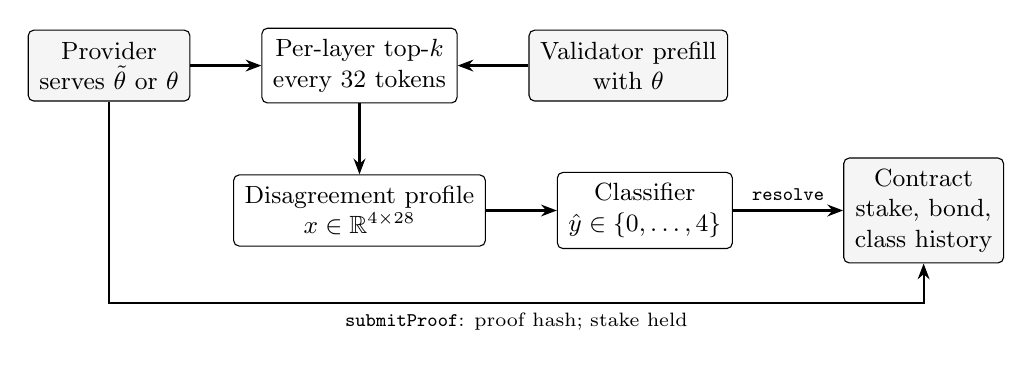
\begin{tikzpicture}[
  node distance=6mm and 9mm,
  box/.style={draw, rounded corners=2pt, align=center, font=\small, inner sep=4pt, minimum height=9mm},
  arr/.style={-{Stealth[length=2mm]}, thick},
  lab/.style={font=\scriptsize, align=center}
]
\node[box, fill=gray!8] (prov) {Provider\\serves $\tilde\theta$ or $\theta$};
\node[box, right=of prov] (proof) {Per-layer \topk{}\\every 32 tokens};
\node[box, right=of proof, fill=gray!8] (val) {Validator prefill\\with $\theta$};
\node[box, below=9mm of proof] (feat) {Disagreement profile\\$x \in \mathbb{R}^{4\times 28}$};
\node[box, right=of feat] (clf) {Classifier\\$\hat y \in \{0,\dots,4\}$};
\node[box, right=14mm of clf, fill=gray!8] (chain) {Contract\\stake, bond,\\class history};
\draw[arr] (prov) -- (proof);
\draw[arr] (val) -- (proof);
\draw[arr] (proof) -- (feat);
\draw[arr] (feat) -- (clf);
\draw[arr] (clf) -- node[lab, above] {\texttt{resolve}} (chain);
\draw[arr] (prov.south) |- node[lab, pos=0.75, below] {\texttt{submitProof}: proof hash; stake held} ([yshift=-5mm]chain.south) -- (chain.south);
\end{tikzpicture}
\caption{Overview. The provider's per-layer \topk{} activations are compared with a validator prefill under the committed weights (\cref{sec:profile}). A classifier turns the profile into a verdict (\cref{sec:classifier}), and an upheld challenge slashes the stake and stores the label (\cref{sec:protocol}).}
\label{fig:overview}
\end{figure*}

\subsection{Per-layer disagreement profile}
\label{sec:profile}

Let $h^{(\ell)}_t \in \mathbb{R}^{1536}$ be the output of decoder layer $\ell \in \{0,\dots,27\}$ at position $t$.
At each checkpoint $t_c = |\text{prompt}| + 32c$ with $c = 0,\dots,7$, we take the indices $I$ and values $v$ of the 128 largest-magnitude entries of $h^{(\ell)}_{t_c}$, for the model under test and for $\theta$ on the same tokens.
For each checkpoint and layer we compute the overlap of the index sets and TOPLOC's three statistics:
\begin{align*}
  f_{\text{idx}} &= 1 - \tfrac{1}{k}\,|\tilde I \cap I|, \\
  f_{\exp} &= \textstyle\sum_{i} \mathbb{1}[\operatorname{exp}(\tilde v_i) \neq \operatorname{exp}(v_i)], \\
  f_{\text{mean}} &= \operatorname{mean}_i |\operatorname{mant}(\tilde v_i) - \operatorname{mant}(v_i)|, \\
  f_{\text{med}} &= \operatorname{median}_i |\operatorname{mant}(\tilde v_i) - \operatorname{mant}(v_i)|.
\end{align*}
Here $\operatorname{exp}$ and $\operatorname{mant}$ are the exponent and mantissa fields of the float32 value, and $i$ runs over rank.
Averaging over the eight checkpoints gives a profile $x \in \mathbb{R}^{4 \times 28}$.
Its last row is what TOPLOC already uses.

\subsection{Classifier and decision rule}
\label{sec:classifier}

We train a multinomial logistic regression with balanced class weights on profiles labelled clean or with one of four modifications, with features standardised on the training data.
A linear model is easy to inspect and needs only a few hundred examples per class.
The predicted class gives attribution.
For the binary verdict we accept a sequence when $P(\text{clean}) \ge \tau$.
The threshold $\tau$ is chosen on training prompts only: we compute out-of-fold $P(\text{clean})$ for honest training sequences by prompt-grouped cross-validation and set $\tau$ at their 1st percentile, a target FRR of 1\%.
Test prompts are never used to choose $\tau$.

\subsection{Verification protocol}
\label{sec:protocol}

\Cref{tab:protocol} separates what we implemented from what a deployment would need.
TOPLOC's last-layer commitment, the validator's recomputation, the classifier and the staking contract are implemented; a per-layer commitment is not integrated into the protocol, and its cost is measured separately (\cref{sec:res-cost}).
In our main experiments the provider side is also a prefill, which isolates the effect of the weights; \cref{sec:res-decode} repeats them with decode-time activations, which is what a provider would commit to.

The contract (142 lines of Solidity) stores each provider's model hash, stake and history of tamper classes, and each proof's prompt hash, proof hash and timestamp.
A challenger posts a bond within two hours of a proof, and only the validator can resolve it.
If upheld, the stake is split between challenger and validator, the bond is returned and the class is recorded (0 clean, 1 8-bit, 2 4-bit, 3 LoRA, 4 fine-tune, 255 unattributed); otherwise the validator keeps the bond.
For a sampling rate $p$, stake $S$ and a saving $\Delta$ per request from tampering, a risk-neutral provider facing certain detection on sampled requests is deterred when $\Delta < pS$.
The system is not trustless: its verdicts are as trustworthy as the validator.

\begin{table*}[!t]
\centering
\small
\caption{Protocol steps, what each relies on, and what we implemented.}
\label{tab:protocol}
\begin{tabular}{@{}>{\raggedright\arraybackslash}p{0.24\textwidth}>{\raggedright\arraybackslash}p{0.27\textwidth}>{\raggedright\arraybackslash}p{0.25\textwidth}>{\raggedright\arraybackslash}p{0.16\textwidth}@{}}
\toprule
Step & Mechanism & Relies on & Status \\
\midrule
Provider commits to activations & TOPLOC polynomial commitment, last layer & cryptographic binding of the proof to its hash & implemented \\
 & per-layer commitment (28 proofs) & same & measured separately, not integrated \\
Commitment bound to the served text & validator recomputes on the served tokens & validator honesty & implemented \\
Commitment bound to the model that generated the text & none & --- & not provided (\cref{sec:security}) \\
Verdict & last-layer thresholds; per-layer classifier & statistical separation, validator honesty & implemented \\
Authorised kernel & declaration or enforcement & not specified & proposed \\
Penalty & stake, bond, dispute window & smart contract; single trusted validator & implemented (local chain) \\
\bottomrule
\end{tabular}
\end{table*}

%=====================================================================
\section{Experimental setup}
\label{sec:setup}

\Cref{tab:setup} lists the setup and \cref{tab:controls} the controls.
Each prompt gets a greedy 256-token answer with the end-of-sequence token suppressed, so every sequence has eight checkpoints; in a 20-prompt probe without suppression, 19 answers ran to 256 tokens anyway.
The two trained modifications see 2{,}400 Alpaca~\cite{taori2023alpaca} examples, with effective batch 8 and sequence length 512.

\begin{table}[!htb]
\centering
\small
\caption{Setup of the main experiments.}
\label{tab:setup}
\begin{tabular}{@{}ll@{}}
\toprule
Model & Qwen2.5-1.5B-Instruct~\cite{qwen2025qwen25}, rev.\ \texttt{989aa79} \\
Shape & 28 layers, hidden size 1536, bf16 \\
Hardware & NVIDIA A10G (24\,GB) \\
Software & PyTorch 2.11, CUDA 12.8, transformers 5.17, \\
 & \texttt{toploc} 0.1.6, TF32 off \\
Prompts & 200 from UltraChat-200k~\cite{ding2023ultrachat} \\
Answers & greedy, 256 tokens, 8 checkpoints \\
Reference & SDPA attention, batch 1 \\
Honest & eager; batch 4; batch 4 + 17 padding \\
Tampered & 4 models (\cref{tab:variants}) \\
Splits & 5-fold CV grouped by prompt, or a \\
 & train/test split by prompt id (stated per table) \\
Threshold & 1\% FRR on training prompts only \\
\bottomrule
\end{tabular}
\end{table}

\begin{table*}[!t]
\centering
\small
\caption{Tampered models. All four write coherent text on a sanity prompt.}
\label{tab:variants}
\begin{tabular}{@{}cll@{}}
\toprule
Class & Variant & Construction \\
\midrule
1 & 8-bit     & bitsandbytes LLM.int8()~\cite{dettmers2022llmint8}, outlier threshold 6.0 \\
2 & 4-bit     & bitsandbytes NF4~\cite{dettmers2023qlora}, bf16 compute \\
3 & LoRA      & $r{=}16$, $\alpha{=}32$ on Q/K/V, lr $2{\times}10^{-4}$, 300 steps, merged~\cite{hu2022lora} \\
4 & Fine-tune & all weights, lr $10^{-5}$, 8-bit AdamW, 300 steps \\
\bottomrule
\end{tabular}
\end{table*}

\begin{table}[!htb]
\centering
\small
\caption{Controls and the confound each addresses.}
\label{tab:controls}
\begin{tabular}{@{}>{\raggedright\arraybackslash}p{0.42\linewidth}>{\raggedright\arraybackslash}p{0.5\linewidth}@{}}
\toprule
Control & Confound \\
\midrule
Grouped by prompt & same prompt in train and test \\
Shared text & classifier learns the text, not the weights \\
Pre-EOS checkpoints & effect of suppressing end of sequence \\
Decode-time activations & prefill on both sides is unrealistic \\
Layer, feature, checkpoint, $k$ ablations & where the signal comes from \\
Held-out modification & closed-set accuracy mistaken for integrity \\
Held-out honest kernel & classifier only knows seen kernels \\
Kernel attack & provider exploits authorised variation \\
\bottomrule
\end{tabular}
\end{table}

%=====================================================================
\section{Results}
\label{sec:results}

\subsection{The last-layer check under honest kernel noise}
\label{sec:res-baseline}

\Cref{tab:recal} shows the check with three sets of thresholds.
Calibrated on all three honest configurations, it keeps a 2\% FPR on held-out prompts but flags no quantised sequence and only 55--60\% of fine-tuned ones.
The published thresholds reject 23\% of honest prompts.
Calibrating without eager traffic gives much tighter thresholds, which flag every tampered sequence but reject all 200 eager prompts and 4\% of the remaining honest traffic.
A second calibration run reproduced the first row exactly.

\begin{table*}[!t]
\centering
\small
\caption{TOPLOC's last-layer check under three sets of thresholds $(T_{\exp}, T_{\text{mean}}, T_{\text{median}})$. FPR is on held-out prompts of the calibration configurations; the other columns cover all 200 prompts.}
\label{tab:recal}
\begin{tabular}{@{}lcccccc@{}}
\toprule
 & & & \multicolumn{4}{c}{Detection (\%) \up} \\
\cmidrule(l){4-7}
Calibrated on & FPR (\%) \down & Eager rejected (\%) \down & 8-bit & 4-bit & LoRA & Fine-tune \\
\midrule
All three configs $(46.02, 25.80, 20.0)$ & \best{2}  & \best{6}  & 0   & 0   & 59.5 & 54.5 \\
Batch-shape only $(7.01, 1.80, 1.0)$    & 4         & 100       & \best{100} & \best{100} & \best{100} & \best{100} \\
Published $(38, 10, 8)$                 & 23        & 69        & 0   & 50  & \best{100} & \best{100} \\
\bottomrule
\end{tabular}
\end{table*}

\Cref{tab:noise} explains why.
On all three statistics, eager attention moves the last layer further than 4-bit quantisation does, and 8-bit quantisation falls between batch-size noise and eager noise.
These results do not contradict TOPLOC's.
Our batch-size noise falls inside the range TOPLOC reports, and the published thresholds raise no false alarms on it.
Eager attention is the outlier: its mantissa statistics are more than twice the largest TOPLOC reports.
Our model is also smaller; with a hidden size of 1536, the 128 recorded entries cover 8.3\% of the hidden state, against at most 3.6\% for the models TOPLOC tested.

\begin{table*}[!t]
\centering
\small
\caption{Last-layer statistics for honest configurations and tampered models, as the mean over 200 prompts of each sequence's maximum. TOPLOC's range spans the maxima in its Table~2~\cite{ong2025toploc}.}
\label{tab:noise}
\begin{tabular}{@{}llccc@{}}
\toprule
 & Source & Exponent mismatches & Mantissa mean & Mantissa median \\
\midrule
\multirow{3}{*}{Honest}   & Eager attention      & \best{25.55} & \best{14.22} & \best{10.64} \\
                          & Batch 4              & 4.35  & 1.35  & 1.00  \\
                          & Batch 4 + 17 padding & 4.30  & 1.37  & 1.02  \\
\midrule
\multirow{4}{*}{Tampered} & 8-bit                & 8.88  & 3.47  & 2.71  \\
                          & 4-bit                & 21.67 & 10.59 & 8.59  \\
                          & LoRA                 & 43.19 & 25.70 & 22.72 \\
                          & Fine-tune            & 41.05 & 24.05 & 20.46 \\
\midrule
\multicolumn{2}{@{}l}{TOPLOC honest range}       & 12--28 & 3.15--6.30 & 2--4 \\
\multicolumn{2}{@{}l}{Published thresholds}      & 38     & 10         & 8    \\
\bottomrule
\end{tabular}
\end{table*}

\subsection{Attribution with the per-layer profile}
\label{sec:res-profile}

With the full profile, the classifier accepts both kernels and still separates the known modifications.
\Cref{tab:confusion} gives the out-of-fold result on matched text, with each honest configuration as a separate example.
Balanced accuracy is 99.3\%; the 95\% $t$-interval across the five folds is 98.7--99.9\%.
This interval reflects variation between prompt folds within one model, GPU and software stack, not variation between deployments.
Per-class precision and recall are at least 0.96 for every class (\cref{tab:perclass}).
Most errors fall on honest eager traffic: 13 of 200 prompts (6.5\%) are labelled as quantised.
\Cref{tab:configs} lists other settings; the pooled one we fixed before the experiment averages each prompt's three honest profiles and scores 99.5\%, but averaging hides the eager errors.

\begin{table*}[!t]
\centering
\small
\caption{Out-of-fold confusion matrix of the per-layer classifier on matched text, prefill on both sides. Rows are the true source; columns are the predicted class.}
\label{tab:confusion}
\begin{tabular}{@{}lccccc@{}}
\toprule
 & Clean & 8-bit & 4-bit & LoRA & Fine-tune \\
\midrule
Honest: eager attention   & \best{187} & 8 & 5 & 0 & 0 \\
Honest: batch 4           & \best{199} & 0 & 0 & 0 & 1 \\
Honest: batch 4 + padding & \best{199} & 0 & 0 & 0 & 1 \\
8-bit                     & 1 & \best{199} & 0 & 0 & 0 \\
4-bit                     & 0 & 0 & \best{200} & 0 & 0 \\
LoRA                      & 0 & 0 & 1 & \best{199} & 0 \\
Fine-tune                 & 0 & 0 & 0 & 0 & \best{200} \\
\bottomrule
\end{tabular}
\end{table*}

\begin{table}[!htb]
\centering
\small
\caption{Per-class precision and recall, same predictions as \cref{tab:confusion}.}
\label{tab:perclass}
\begin{tabular}{@{}lccc@{}}
\toprule
Class & Precision \up & Recall \up & Support \\
\midrule
Clean     & 0.998 & 0.975 & 600 \\
8-bit     & 0.961 & 0.995 & 200 \\
4-bit     & 0.971 & 1.000 & 200 \\
LoRA      & 1.000 & 0.995 & 200 \\
Fine-tune & 0.990 & 1.000 & 200 \\
\bottomrule
\end{tabular}
\end{table}

\begin{table*}[!t]
\centering
\small
\caption{Five-class balanced accuracy (\%) by setting, with the 95\% interval across the five folds. Separate: one honest example per configuration (main setting). Pooled: the three honest configurations averaged per prompt, as fixed before the experiment.}
\label{tab:configs}
\begin{tabular}{@{}llccc@{}}
\toprule
Text & Checkpoints & LR, separate \up & LR, pooled \up & $k$-NN, pooled \up \\
\midrule
Matched & all eight & \best{99.3} {\scriptsize(98.7--99.9)} & 99.5 {\scriptsize(99.1--99.9)} & 98.8 \\
Matched & pre-EOS   & ---  & 98.8 {\scriptsize(97.4--100)} & 96.7 \\
Shared  & all eight & 99.1 {\scriptsize(98.5--99.6)} & 99.8 {\scriptsize(99.5--100)} & 98.3 \\
Shared  & pre-EOS   & ---  & 98.8 {\scriptsize(97.4--100)} & 97.3 \\
\bottomrule
\end{tabular}
\end{table*}

\begin{figure*}[!t]
\centering
\begin{minipage}[t]{0.49\linewidth}
  \centering
  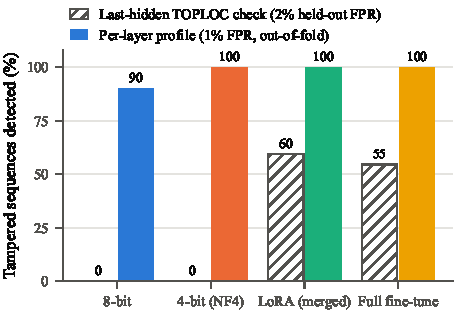
\includegraphics[width=\linewidth]{figures/detection.pdf}
  \caption{Detection rate. Hatched: last-layer check with thresholds calibrated on all honest configurations. Solid: per-layer classifier at 1\% FPR, out of fold.}
  \label{fig:detection}
\end{minipage}\hfill
\begin{minipage}[t]{0.49\linewidth}
  \centering
  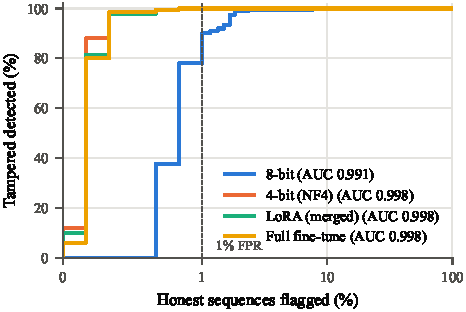
\includegraphics[width=\linewidth]{figures/roc.pdf}
  \caption{ROC of the score $1-P(\text{clean})$ for all honest sequences against each known modification.}
  \label{fig:roc}
\end{minipage}
\end{figure*}

\subsection{Controls and ablations}
\label{sec:res-ablation}

A tampered model writes different text, and the classifier might learn the text.
When both models read identical tokens (shared text) balanced accuracy is 99.1\%, and using only checkpoints before the natural end of the answer gives 98.8\% in both settings (\cref{tab:configs}).

\Cref{fig:ablation} retrains the classifier on parts of the profile.
The last layer alone, the information TOPLOC uses, gives 78.0\%, flagging 74.5\% of eager traffic and missing 27\% of 8-bit sequences.
The first 14 layers give 98.6\% and the last 14 only 91.6\%.
The classifier's weights agree (\cref{fig:coef}): layers 0--4 carry 28\% of the absolute standardised coefficient mass and layer 27 another 7\%, against 3.6\% for a uniform split.
Index overlap and mantissa median carry most of it (31\% each).
Smaller $k$ costs accuracy: 96.2\% at $k{=}16$, 98.4\% at 32, 98.6\% at 64 and 99.3\% at 128, mainly through more eager false alarms (12.5\% at $k{=}16$ against 6.5\% at 128).

\begin{figure}[!htb]
\centering
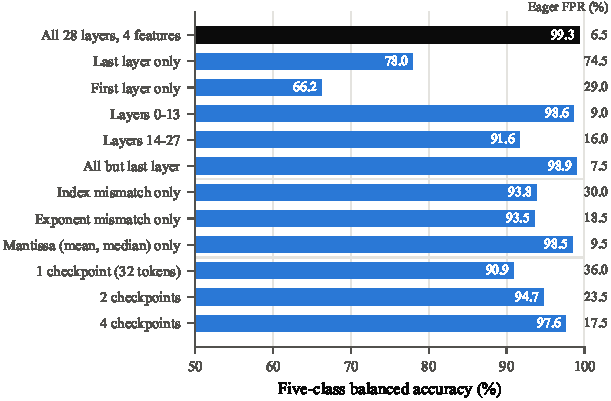
\includegraphics[width=\linewidth]{figures/ablation.pdf}
\caption{Ablations on matched text. Bars show five-class balanced accuracy; the right column shows the share of eager-attention prompts flagged.}
\label{fig:ablation}
\end{figure}

\begin{figure}[!htb]
\centering
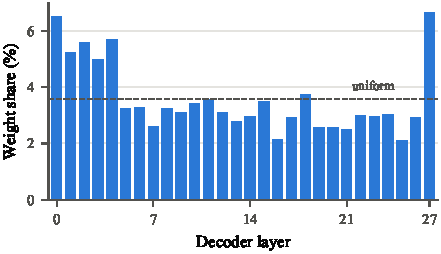
\includegraphics[width=\linewidth]{figures/coef.pdf}
\caption{Share of the classifier's absolute standardised coefficients per layer, summed over classes and features.}
\label{fig:coef}
\end{figure}

\subsection{Decode-time activations}
\label{sec:res-decode}

A real provider would commit to activations recorded while decoding.
We repeated the experiment with the provider side taken from decoding: each tampered model's own generations and teacher-forced decoding for the honest configurations.
We added a fourth honest configuration, the reference model decoding on the reference kernel, so that the honest class includes the decode--prefill gap.
The validator side stays a prefill with $\theta$.

Cross-validated balanced accuracy is 99.0\% (98.4--99.6\%), against 80.6\% for the last layer alone (\cref{tab:decode}).
None of the reference model's own decodes is flagged; eager traffic is flagged on 12\% of prompts.
A classifier trained only on prefill profiles also works on decode-time profiles without retraining, at 99.2\%.

\begin{table*}[!t]
\centering
\small
\caption{Per-layer classifier with the provider's activations recorded during decoding, 200 prompts per source. Out of fold except in the last row.}
\label{tab:decode}
\begin{tabular}{@{}lccccc@{}}
\toprule
 & Balanced & \multicolumn{2}{c}{Honest flagged (\%) \down} & \multicolumn{2}{c}{Detected at 1\% FPR (\%) \up} \\
\cmidrule(lr){3-4}\cmidrule(l){5-6}
Training data & accuracy (\%) \up & Ref.\ decode & Eager & 8-bit & 4-bit / LoRA / FT \\
\midrule
Decode, all layers               & \best{99.0} {\scriptsize(98.4--99.6)} & 0 & 12 & 85 & 100 \\
Decode, last layer only          & 80.6 {\scriptsize(79.7--81.5)} & 0 & 90 & --- & --- \\
Prefill only (no retraining)     & 99.2 & 0 & 3 & --- & --- \\
\bottomrule
\end{tabular}
\end{table*}

\subsection{Operating point}
\label{sec:res-op}

Balanced accuracy averages over classes and decision rules; a verifier needs FAR and FRR at one threshold.
\Cref{tab:op} trains on prompts 0--99, chooses $\tau$ on those prompts only, and tests on prompts 100--199.
Intervals are Wilson 95\% intervals with the sequence as the sampling unit.
At the 1\% FRR target the verifier rejects 0.7\% of honest prefill sequences but accepts 47\% of 8-bit sequences; 4-bit, LoRA and fine-tune are never accepted.
On decode-time data the 8-bit FAR falls to 22\% at an FRR of 1.8\%.
Taking the most likely class instead of thresholding $P(\text{clean})$ accepts no 8-bit prefill sequence but rejects 4.3\% of honest ones.
8-bit quantisation is the binding case: its profile is the one closest to honest eager traffic, so any operating point trades 8-bit acceptance against eager rejection.
$P(\text{clean})$ is reasonably calibrated on the test split (expected calibration error 0.021, Brier score 0.015).

\begin{table*}[!t]
\centering
\small
\caption{Verdicts at a fixed threshold. Train prompts 0--99, test prompts 100--199 (100 per source); $\tau$ set for 1\% FRR on training prompts. FRR: honest sequences rejected. FAR: tampered sequences accepted. Brackets: Wilson 95\% intervals.}
\label{tab:op}
\begin{tabular}{@{}lccccc@{}}
\toprule
 & FRR (\%) \down & \multicolumn{4}{c}{FAR (\%) \down} \\
\cmidrule(l){3-6}
Provider activations & all honest & 8-bit & 4-bit & LoRA & Fine-tune \\
\midrule
Prefill, threshold   & 0.7 \ci{0.2}{2.4} & 47 \ci{37.5}{56.7} & 0 \ci{0}{3.7} & 0 \ci{0}{3.7} & 0 \ci{0}{3.7} \\
Prefill, most likely class & 4.3 \ci{2.5}{7.3} & 0 \ci{0}{3.7} & 0 \ci{0}{3.7} & 0 \ci{0}{3.7} & 0 \ci{0}{3.7} \\
Decode, threshold    & 1.8 \ci{0.9}{3.6} & 22 \ci{15.0}{31.1} & 0 \ci{0}{3.7} & 0 \ci{0}{3.7} & 0 \ci{0}{3.7} \\
Decode, most likely class & 3.2 \ci{1.9}{5.5} & 3 \ci{1.0}{8.5} & 0 \ci{0}{3.7} & 0 \ci{0}{3.7} & 0 \ci{0}{3.7} \\
\bottomrule
\end{tabular}
\end{table*}

\subsection{Unknown modifications}
\label{sec:res-open}

A verifier must reject modifications it was never trained on.
We left each known modification out of training in turn and tested whether it is accepted as clean (\cref{tab:open}).
Held-out 4-bit, LoRA and fine-tuned sequences are still rejected, with at most 1 of 100 accepted; the classifier simply gives them a neighbouring label.
Held-out 8-bit quantisation is accepted on all 100 test prompts, with prefill or decode-time data.
The classifier separates 8-bit from clean only because it has seen 8-bit; it does not learn a general notion of ``not $\theta$''.

We also served six modifications that never appeared in training (\cref{tab:newmods}): the LoRA model loaded with 4-bit weights, and 4-bit quantisation of only some layers (the first 14, the last 14, even layers, odd layers, or only the MLPs).
These share 4-bit quantisation with a training class, so they test variation around a known modification rather than an unrelated one.
With the detector restricted to SDPA traffic, none of the 300 test sequences was accepted.
The detector that also accepts eager traffic accepted 4 of 50 sequences quantised in the first 14 layers.
The mixed-kernel last-layer check caught 66\% of the LoRA model but at most 2\% of the partial quantisations.

\begin{table*}[!t]
\centering
\small
\caption{Modifications never seen in training, test prompts 150--199 (50 sequences each), decode-time activations, threshold rule. Detectors trained on prompts 0--149. Brackets: Wilson 95\% intervals.}
\label{tab:newmods}
\begin{tabular}{@{}lcccccc@{}}
\toprule
 & Share of linear & \multicolumn{2}{c}{Per-layer FAR (\%) \down} & \multicolumn{3}{c}{Last-layer detected (\%) \up} \\
\cmidrule(lr){3-4}\cmidrule(l){5-7}
Modification & params in 4-bit & Unrestricted & SDPA only & All configs & Batch-shape only & Published \\
\midrule
LoRA + 4-bit          & 100\% & 0 \ci{0}{7.1} & 0 \ci{0}{7.1} & 66 & 100 & 100 \\
4-bit, layers 0--13   & 50\%  & 8 \ci{3.2}{18.8} & 0 \ci{0}{7.1} & 0 & 100 & 26 \\
4-bit, layers 14--27  & 50\%  & 0 \ci{0}{7.1} & 0 \ci{0}{7.1} & 0 & 100 & 16 \\
4-bit, even layers    & 50\%  & 0 \ci{0}{7.1} & 0 \ci{0}{7.1} & 0 & 100 & 10 \\
4-bit, odd layers     & 50\%  & 0 \ci{0}{7.1} & 0 \ci{0}{7.1} & 2 & 100 & 12 \\
4-bit, MLPs only      & 88\%  & 0 \ci{0}{7.1} & 0 \ci{0}{7.1} & 2 & 100 & 40 \\
\bottomrule
\end{tabular}
\end{table*}

\begin{table}[!htb]
\centering
\small
\caption{Held-out modification accepted as clean (FAR, \%), threshold rule, test prompts 100--199, 100 sequences each, with Wilson 95\% intervals. FRR on honest test traffic was 0.5--1.8\%.}
\label{tab:open}
\begin{tabular}{@{}lcc@{}}
\toprule
Held out & Prefill & Decode \\
\midrule
8-bit     & 100 \ci{96.3}{100} & 100 \ci{96.3}{100} \\
4-bit     & 1 \ci{0.2}{5.4}    & 1 \ci{0.2}{5.4} \\
LoRA      & 0 \ci{0}{3.7}      & 0 \ci{0}{3.7} \\
Fine-tune & 0 \ci{0}{3.7}      & 0 \ci{0}{3.7} \\
\bottomrule
\end{tabular}
\end{table}

\subsection{Configuration-adaptive provider (A2)}
\label{sec:res-attack}

Because eager traffic counts as honest, a provider can tamper with the weights and serve the result with eager attention.
We replayed each tampered model's own generations by decoding, with eager attention at batch 1 and with SDPA at batch 4, on prompts 100--199.

\Cref{tab:attack} uses a classifier trained on decode-time data from prompts 0--99 without attack examples, taking the most likely class.
Eager attention hides the quantisation: 77\% of 8-bit and 66\% of 4-bit sequences are called clean, and LoRA and fine-tuned sequences, though still flagged on 71--78\% of prompts, usually get the wrong label.
The last-layer check with mixed-kernel thresholds catches only 12\% of eager-served 8-bit.
Batch 4 does not help the attacker; 96--100\% of those sequences are caught and correctly named.

\begin{table*}[!t]
\centering
\small
\caption{Tampered models served with a non-reference kernel, 100 held-out prompts each. Per-layer: most likely class from a classifier trained on decode-time data from prompts 0--99 without attack examples. Last-layer: the thresholds of \cref{tab:recal}.}
\label{tab:attack}
\begin{tabular}{@{}llccccc@{}}
\toprule
 & & \multicolumn{2}{c}{Per-layer (\%)} & \multicolumn{3}{c}{Last-layer detected (\%) \up} \\
\cmidrule(lr){3-4}\cmidrule(l){5-7}
Kernel & Variant & Detected \up & Called clean \down & All configs & Batch-shape only & Published \\
\midrule
\multirow{4}{*}{Eager, batch 1} & 8-bit     & 23 & 77 & 12 & 100 & 77  \\
                                & 4-bit     & 34 & 66 & 64 & 100 & 99  \\
                                & LoRA      & 71 & 29 & 91 & 100 & 100 \\
                                & Fine-tune & 78 & 22 & 77 & 100 & 100 \\
\midrule
\multirow{4}{*}{SDPA, batch 4}  & 8-bit     & \best{96}  & 4 & 0  & 100 & 1   \\
                                & 4-bit     & \best{100} & 0 & 0  & 100 & 50  \\
                                & LoRA      & \best{100} & 0 & 59 & 100 & 100 \\
                                & Fine-tune & \best{100} & 0 & 57 & 100 & 100 \\
\bottomrule
\end{tabular}
\end{table*}

\paragraph{Kernel policy.}
\Cref{tab:policy} compares three policies at the threshold rule, training on prompts 0--149 and testing on 150--199 (50 sequences per cell).
Under the \emph{unrestricted} policy, one detector accepts every authorised kernel; it accepts 92\% of eager-served 8-bit and 68\% of eager-served 4-bit.
Under a \emph{declared} policy, each provider names its kernel and the verifier uses a detector trained for that kernel, including on eager-served tampering; the attacker declares whichever kernel is accepted more often.
This catches eager-served 4-bit, LoRA and fine-tuning (accepted on 2--8\% of prompts) while rejecting 2\% of honest eager traffic, but it still accepts 96\% of eager-served 8-bit.
A declaration is also only a claim: nothing in our protocol checks it.
Under an \emph{enforced} policy, the provider must serve with SDPA; the verifier then accepts none of the 400 tampered test sequences, at the default batch or at batch 4, and rejects none of the 150 honest ones.
With 50 sequences per cell, the 95\% upper bound on each of these zero rates is 7.1\%.
In this experiment the validator's reference is always an SDPA prefill, since we did not record eager reference prefills.
Adding attack examples to a single detector for all kernels instead raises eager-attack detection to 62\% for 8-bit and 98--100\% for the others, but it then flags 38\% of honest eager traffic.

\begin{table*}[!t]
\centering
\small
\caption{Kernel policies, threshold rule, test prompts 150--199 (50 sequences per cell). FAR on eager-served tampering; under the declared policy the attacker's better declaration is shown. Brackets: Wilson 95\% intervals.}
\label{tab:policy}
\begin{tabular}{@{}lcccccc@{}}
\toprule
 & \multicolumn{2}{c}{FRR (\%) \down} & \multicolumn{4}{c}{FAR on eager-served tampering (\%) \down} \\
\cmidrule(lr){2-3}\cmidrule(l){4-7}
Policy & eager & SDPA configs & 8-bit & 4-bit & LoRA & Fine-tune \\
\midrule
Unrestricted & 4 \ci{1.1}{13.5} & 0 \ci{0}{7.1} & 92 \ci{81.2}{96.8} & 68 \ci{54.2}{79.2} & 28 \ci{17.5}{41.7} & 28 \ci{17.5}{41.7} \\
Declared     & 2 \ci{0.4}{10.5} & 0 \ci{0}{7.1} & 96 \ci{86.5}{98.9} & 6 \ci{2.1}{16.2} & 2 \ci{0.4}{10.5} & 8 \ci{3.2}{18.8} \\
Enforced SDPA & not allowed & 0 \ci{0}{7.1} & \multicolumn{4}{c}{not possible; SDPA-served tampering: 0 \ci{0}{7.1} for all 8 attacks} \\
\bottomrule
\end{tabular}
\end{table*}

\paragraph{Unseen honest kernels.}
The classifier only accepts kernels it has seen.
Left out of training, a batch-size configuration is still accepted (0.5\% flagged), but all 200 eager prompts are flagged, mostly as 4-bit.
A small honest-only check on an NVIDIA L4 raised no false alarms on 50 sequences under either check; we did not run tampered models on the L4.

\subsection{Detector-guided quantisation (A3)}
\label{sec:res-aware}

An attacker who can query the detector can choose what to quantise.
We gave the attacker the five partial quantisations of \cref{tab:newmods}, each covering at least half of the linear parameters, and let it score them on calibration prompts 0--19 with the detector it faces, picking the one accepted most often (ties broken by mean $P(\text{clean})$).
Against the SDPA-only detector no candidate was accepted on any calibration prompt; the search picked the last-14-layer variant, which was accepted on 0 of 50 test prompts.
Against the detector that also accepts eager traffic, the search picked the first-14-layer variant (accepted on 1 of 20 calibration prompts), which was accepted on 4 of 50 test prompts (8\%, \ci{3.2}{18.8}).
This is a weak attacker with five discrete choices, and it does not show robustness to an attacker that optimises the weights against the detector.


\subsection{A second model}
\label{sec:res-smol}

We repeated the core experiment on SmolLM2-1.7B-Instruct, a Llama-architecture model from a different family (24 layers, hidden size 2048, revision \texttt{31b70e2}), with 100 prompts, 128-token answers and decode-time activations.
Honest traffic was the reference decode, eager attention and batch 4; tampered traffic was 4-bit and 8-bit quantisation, and the eager attack used prompts 50--99.

The picture differs from Qwen (\cref{tab:smol}).
Eager attention barely changes this model: its mean index mismatch is within 0.002 of the reference decode at every layer, while 8-bit and 4-bit sit at 0.08--0.12 and 0.14--0.22 respectively across layers.
The full profile reaches 98.7\% balanced accuracy and the last layer alone 98.4\%; no honest sequence is flagged and no tampered sequence is called clean in cross-validation.
At the threshold rule, trained on prompts 0--49 and tested on 50--99, eager-served quantisation is never accepted, and a detector trained without eager traffic still accepts all honest eager traffic.
On this model, then, there is no kernel loophole and no need for the full profile.
Whether a model shows the overlap seen on Qwen has to be measured per model.

\begin{table}[!htb]
\centering
\small
\caption{SmolLM2-1.7B-Instruct, decode-time activations. CV: 5-fold grouped by prompt, 100 prompts. FAR and FRR: train prompts 0--49, test 50--99 (50 per cell), threshold rule, detector accepting all honest configurations.}
\label{tab:smol}
\begin{tabular}{@{}lc@{}}
\toprule
Balanced accuracy, all 24 layers (CV) & 98.7\% \\
Balanced accuracy, last layer only (CV) & 98.4\% \\
FRR: reference / eager / batch 4 & 0 / 0 / 2\% \\
FAR: 4-bit / 8-bit & 0 / 0\% \\
FAR: eager-served 4-bit / 8-bit & 0 / 0\% \\
\bottomrule
\end{tabular}
\end{table}


\subsection{Cost}
\label{sec:res-cost}

\paragraph{Commitment.}
We built real TOPLOC commitments for all 28 layers of 10 reference generations (256 tokens each, $k{=}128$).
One commitment per layer takes 2{,}064 bytes per sequence, the same as TOPLOC's last-layer commitment, so the full profile costs 57{,}792 bytes per 256 tokens, or 226 bytes per token.
Building all 28 commitments took 0.22\,s and verifying them 0.29\,s per sequence on the instance's CPU, and capturing every layer during the validator's prefill added no measurable time to its 0.042\,s.
We did not integrate these commitments into the contract or measure them under load.

\paragraph{Serving.}
\Cref{tab:throughput} shows decoding throughput at three batch sizes.
At batch 1, 8-bit is $4.9\times$ and 4-bit $1.3\times$ slower than bf16, as in our earlier measurement, so the time saving $\Delta$ is negative.
At batch 32, 4-bit reaches 96\% of bf16 throughput with 29\% less peak memory, which leaves room for more replicas or larger batches per GPU; 8-bit stays three times slower.
Whether cheating pays therefore depends on the serving load, and the condition $\Delta < pS$ has to be evaluated at the provider's own operating point.

\begin{table}[!htb]
\centering
\small
\caption{Decoding throughput (tokens/s, all sequences) and peak memory on an A10G, 128 new tokens, mean of two runs after one warm-up.}
\label{tab:throughput}
\begin{tabular}{@{}lccc@{}}
\toprule
Batch & bf16 & 8-bit & 4-bit \\
\midrule
1  & 39.1 & 8.0   & 29.4 \\
8  & 258.3 & 55.3 & 203.1 \\
32 & 494.2 & 163.9 & 476.5 \\
\midrule
Peak MiB, batch 32 & 6209 & 6236 & 4413 \\
\bottomrule
\end{tabular}
\end{table}


We also ran the whole pipeline once on a local Anvil chain: a provider staked 100 mock tokens and served the fine-tuned model, the last-layer check flagged the sequence (57 exponent mismatches against 46.02), the classifier returned class 4, and the contract zeroed the stake and recorded \texttt{[4]}.

%=====================================================================
\section{Security analysis}
\label{sec:security}

\paragraph{What the 99.3\% measures.}
It is closed-set attribution among four modifications, in one model, on one GPU type, with prompt folds as the only source of variation.
It does not bound the acceptance of unknown modifications, which can be complete (\cref{sec:res-open}), and the fold interval is not a deployment interval.

\paragraph{Commitments and selective disclosure.}
A TOPLOC commitment binds activations to the tokens the validator recomputes, so a provider cannot report activations that do not match those tokens under $\theta$.
It does not bind the tokens to the weights that chose them.
A provider can generate with $\tilde\theta$, then run one prefill with $\theta$ on its own output and commit to those activations; both checks then pass.
This costs one prefill per sampled response, far less than generation, and it is the same gap TOPLOC reports for speculative decoding.
Closing it needs a binding between sampling and the committed weights, for example output-distribution tests on the served text~\cite{gao2025model} or trusted execution~\cite{cai2025auditing}.
A provider that serves verification requests differently from ordinary ones is also outside what any per-response check can see, unless verification requests are indistinguishable from traffic.

\paragraph{Kernel enforcement.}
Enforcing the kernel closed the A2 attack in our data, but we have not shown how to enforce it.
A declared kernel is a claim; verifying it needs either a kernel signature in the activations, which our eager results suggest exists but which an attacker could imitate, or attested execution.
Other execution choices we did not vary, such as precision, continuous batching and tensor parallelism, could open similar gaps.

\paragraph{Detector-aware attacks.}
Our A3 attacker searches over a small, discrete set of layer subsets.
An attacker that optimises the weights directly against a known linear detector, for example by fine-tuning with a penalty on the detector's score, is likely to do better, and we did not test it.

\paragraph{Generalisation and statistics.}
Our evidence covers two models of 1.5--1.7B parameters, one GPU type for tampering, and 50--200 prompts per source.
The second model behaved differently from the first, so neither the kernel loophole nor the value of the full profile can be assumed for a new model.
Wilson intervals on 50--100 sequences cannot certify rates below a few percent; a zero count out of 50 only bounds the rate below 7.1\%.

%=====================================================================
\section{Conclusion}
\label{sec:conclusion}

Honest kernel noise and weight tampering can look the same at the last layer of a language model and still differ across its depth.
On Qwen2.5-1.5B-Instruct, a per-layer profile of TOPLOC's statistics attributes four known modifications with 99.3\% balanced accuracy while accepting two attention kernels, where the last-layer check with mixed-kernel thresholds catches no quantisation.
The profile is not an integrity guarantee.
It accepts an unseen 8-bit model on every test prompt, a provider that switches to eager attention passes on most quantised prompts, and neither check binds the served text to the weights that generated it.
With the kernel enforced, no tested attack passed, including six unseen modifications and a detector-guided choice of layers, which suggests that verification protocols should fix the execution configuration rather than tolerate it.
On SmolLM2-1.7B the overlap between kernel noise and quantisation did not occur, so the need for a per-layer profile is a property of the model, to be measured before deployment.
A per-layer commitment is cheap to build and check, but it is 28 times larger than TOPLOC's.
\Cref{tab:status} summarises what is established.

\begin{table}[!htb]
\centering
\small
\caption{Status of the paper's claims.}
\label{tab:status}
\begin{tabular}{@{}>{\raggedright\arraybackslash}p{0.5\linewidth}>{\raggedright\arraybackslash}p{0.44\linewidth}@{}}
\toprule
Claim & Status \\
\midrule
Last-layer check misses quantisation under mixed-kernel thresholds & measured \\
Per-layer attribution of 4 known modifications & measured \\
Holds for decode-time activations & measured \\
Rejects unknown modifications & not established (fails for 8-bit) \\
Robust to kernel choice (A2) & not established \\
Kernel enforcement closes A2 & measured if enforced; enforcement proposed \\
Robust to detector-aware attacks (A3) & one discrete search: no evasion with enforced kernel; weight optimisation untested \\
Other models and hardware & second model: attribution holds, loophole absent; tampering on other GPUs untested \\
Per-layer commitment is practical & commitment measured; not integrated \\
Penalty enforcement & implemented, trusted validator \\
\bottomrule
\end{tabular}
\end{table}

\bibliographystyle{plainnat}
\bibliography{refs}

%=====================================================================
\appendix
\section{Reproducibility}

\begin{itemize}
  \item Code and data: \url{https://github.com/bruce249/proof-of-weights}.
  \item Model revision:\\ {\footnotesize\texttt{989aa7980e4cf806f80c7fef2b1adb7bc71aa306}}.
  \item \texttt{toploc} 0.1.6, PyTorch 2.11.0, transformers 5.17.0.
  \item Seeds: prompts and classifier 20260923, LoRA 202609231, fine-tune 202609232.
  \item Main tables: \texttt{paper/analysis.py}, \texttt{paper/decode\_analysis.py}, \texttt{paper/review\_analysis.py}, \texttt{paper/review\_gpu\_analysis.py}; GPU runs: \texttt{inference/task02.py}, \texttt{task04.py}, \texttt{recalibrate.py}, \texttt{kernel\_attack.py}, \texttt{review\_gpu.py}.
  \item Proofs are built from CPU copies of the activations, because the library failed on CUDA tensors in our environment.
  \item The thresholds, classifier settings and pooled clean class were fixed before the experiments. All other analyses, including every result in \cref{sec:res-op,sec:res-open,sec:res-attack}, were added afterwards and are exploratory.
\end{itemize}

\end{document}
